\section{Geschäftsidee}


\subsection{Motivation}
Eine Studie von International Data Corporation (IDC, eines der führenden Marktforschungsunternehmen in der IT-Industrie) aus dem Jahr 2005\footnote[1]{\textit{White Paper on Hidden Cost of Information Work}, IDC, 2005.} hat gezeigt, dass ein Wissensarbeiter im Durchschnitt rund ein Viertel seiner Arbeitszeit alleine auf die Informationssuche aufwendet. In der wissenschaftlichen Forschung ist dieser Anteil unseren Schätzungen zufolge noch größer. Gesucht wird dabei vor allem nach Information in Form von wissenschaftlichen Publikationen. Weil Publikationen im Idealfall den Stand der Technik abbilden, ist deren Studium ein Grundpfeiler erfolgreicher wissenschaftlicher Praxis. 

\begin{table}[h!]
  \centering
  \begin{large}
  \begin{tabular}{c}\hline
	\\
  {\color{orange}„Wenn ich weiter geblickt habe, so deshalb,} \\ 
	{\color{orange}weil ich auf den Schultern von Riesen stehe.“} \\
	{\hfill \color{orange}\textit{Isaac Newton, 1676} } \\
	\\\hline
  \end{tabular}
  \end{large}
\end{table}

Neben den obligatorischen Veröffentlichungen in Journals und Konferenzbändern bergen Blogs und Magazine häufig eine nicht minder wichtige Quelle für Ideen und neue Sichtweisen. An dieser Stelle kommen allerdings drei wichtige Faktoren ins Spiel, die eine erfolgreiche Literaturrecherche erheblich erschweren: 

\begin{description}
  \item[Wachsendes Informationsuniversum] \hfill \\
  Die Anzahl möglicher Quellen und potentiell wertvoller Informations-Items steigt rasant: 
In 2008 erschienen allein in den acht großen Wissenschaftsnationen 760.671 Veröffentlichung. Selbst bei der gegenwärtigen jährlichen Wachstumsrate von 3,26\% wird sich diese Zahl in zwanzig Jahren verdoppeln. 
  \item[Second] \hfill \\
  The second item
  \item[Third] \hfill \\
  The third etc \ldots
\end{description}

Die Geschäftsidee basiert sich auf starke Notwendigkeit die Zeit für wissenschaftliche Informationssuche zu reduzieren. In moderne Welt, die Zeitaufwand für Informationssuche und Informationsverwaltung steigt enorm zu. In der Studie von IDC, 2005 "White Paper on Hidden Cost of Information Work" haben sie festgestellt, dass ein Mitarbeiter durchschnittlich 9.5 Student pro ein Woche für Informationssuche braucht. Dieser Zeit entspricht ca. 24 \% von gesamte Arbeitszeit. Vorher genutzte Suchverfahren, wie einfache Schlüsselwortsuche, ist sehr schwierig zu automatisieren und verwalten. Die Schlüsselwortsuche ergibt auch nicht vollständige Information, besonderes wenn um wissenschaftliche Suche geht und Definition von Schlüsselworte ist schwierig.


\begin{table}[h!]
  \centering
  \begin{large}
  \begin{tabular}{c}\hline
  \\
  {\color{orange}ein Mitarbeiter braucht durchschnittlich }\\
  {\color{orange}9.5 Student pro ein Woche für Informationssuche}\\
  \\\hline
  \end{tabular}
  \end{large}
\end{table}


Technologien von Semantic Web erlauben nicht nur Suche nach Wörter, sondern nach der Bedeutung der Suchbegriff. Dieser Technologien lassen auch schon gesuchte Information analysieren und auf dieses Basis weiter Suche anpassen und verwalten.

\subsection{Know-how Träger}
Die Know-how wurde bei zwei Studenten der Karlsruher Institut für Technologie (KIT) entwickelt. Artem Schumilin studiert Wirtschaftsingenieurwesen (M.Sc) und Igor Tseyzer studiert Informationswirtschaft (B.Sc). Wahrend des Studiums am KIT haben beide Gründer notwendige Kenntnisse in Bereich Web Technologien und Semantic Web Technologien bekommen, was als stabile Fundament für Bau und weiter Entwicklung der Know-How dienen sollen. 


\subsection{Innovation}

SemLit analysiert alle Informationen aus große Menge der Quellen, die für wissenschaftliche Suche relevant sind. Sie sind vor allem Journale, Zeitschriften, Konferenzen und Blogs. Auf Grund von dieser Datenquellen wird ein semantische Indexierung gemacht und für Endkunden bereitgestellt. Von andere Seite sammelt SemLit Suchanfrage von Endnutzern und macht eine semantische Suche in indexierte Datenbank. Es gibt auch die Möglichkeit vorherige Suchanfrage zu analysieren und Suchergebnisse entsprechend anpassen. Die Funktionsschema von SemLit ist auf Abbildung \ref{fig:idea} dargestellt.
\begin{figure}[h!]
\centering
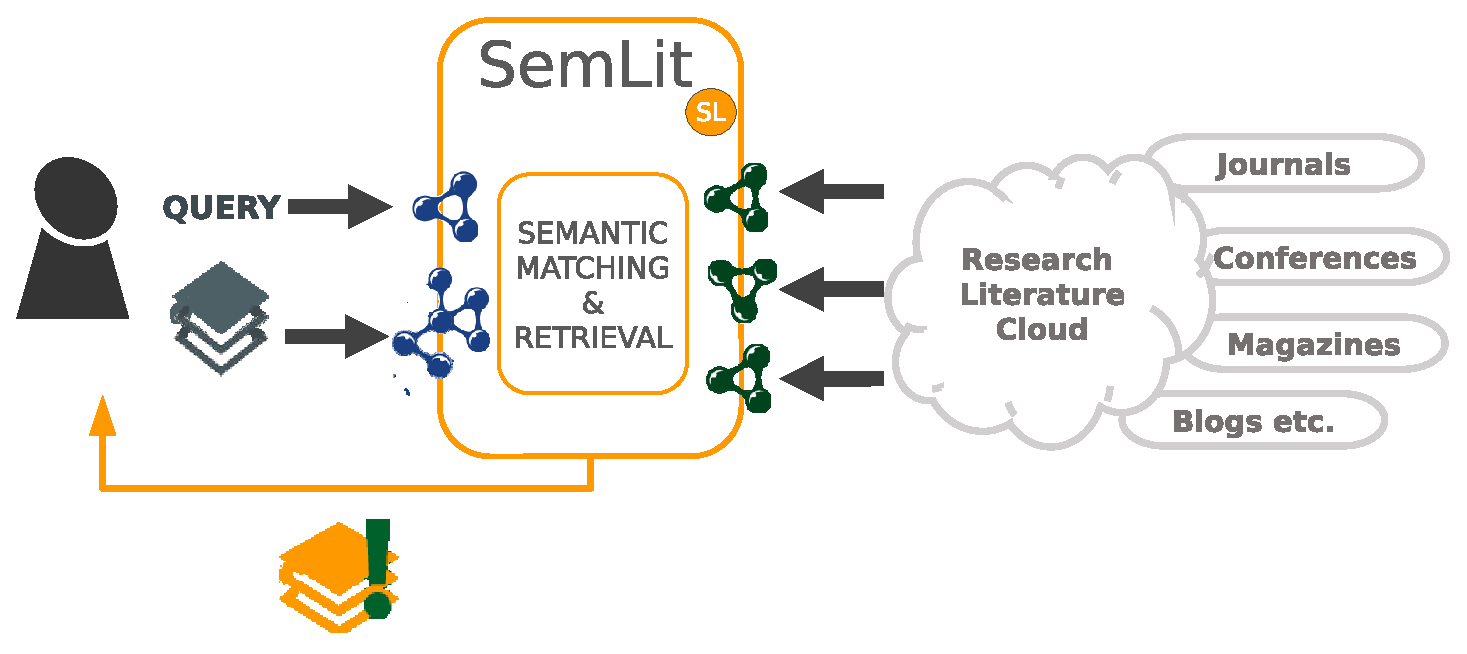
\includegraphics[width=0.9\textwidth]{idea}
\caption{Funktionsschema von SemLit}
\label{fig:idea}
\end{figure}

\subsection{Projektplanung}

SemLit ist in zwei Formen verfügbar: Webauftritt und App für Mobile Geräte. Das Mockup für Webauftritt und Mobile APP können in Abbildung \ref{fig:web} und \ref{fig:app} gesehen werden.

\begin{figure}[h!]
\centering
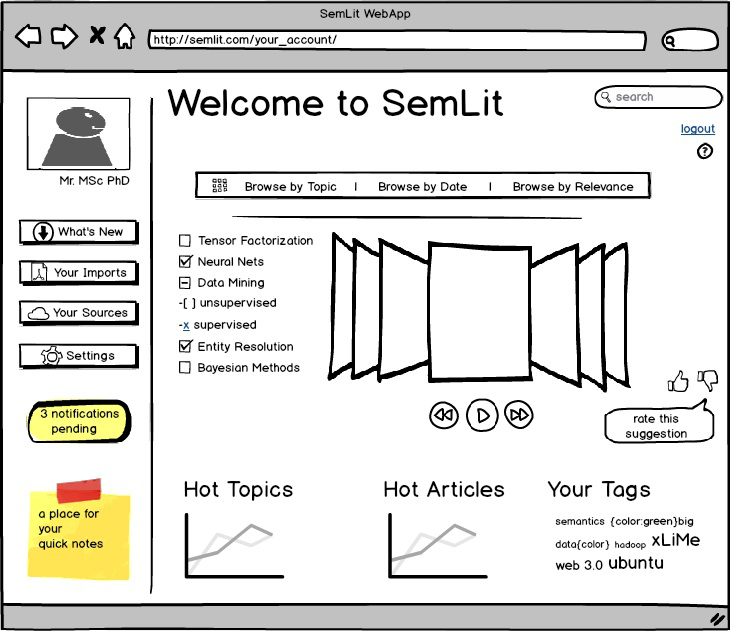
\includegraphics[width=0.6\textwidth]{mockup_web}
\caption{Mockup für Webauftritt}
\label{fig:web}
\end{figure}

\begin{figure}[h!]
\centering
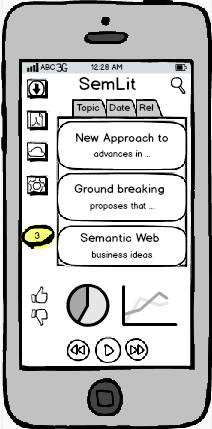
\includegraphics[width=0.2\textwidth]{mockup_app}
\caption{Mockup für Mobile App}
\label{fig:app}
\end{figure}

Die Beide Formen sind Benutzer freundlich und stellen eine Möglichkeit schnell und ohne zusätzliche Aufwand gewünschte Information suchen und verwalten.\\


